\documentclass[aps,prd,twocolumn,nofootinbib]{revtex4-1}
\usepackage{amsmath}
\usepackage{graphicx}
\usepackage{subfig}
\usepackage{epsfig}
\usepackage{listings}
\usepackage[hidelinks,hyperfootnotes=false,bookmarks=false]{hyperref}
\usepackage[colorinlistoftodos]{todonotes}
\usepackage{verbatim}

%\usepackage[section]{placeins}
\usepackage{float}

\DeclareRobustCommand{\su3flavor}{$\text{SU(3)}_{\text{flavor}}$}
\DeclareRobustCommand{\qqbar}{$q\overline{q}$}

\begin{document}

\title{Mesons Beyond \su3flavor \qqbar}
\author{Douglas Davis}
\author{Matthew Epland}
\author{Justin Raybern}
\author{Pingchuan Zhao}
\affiliation{Department of Physics, Duke University, Durham, NC 27707, USA}
\date{\today}
\begin{abstract}
%\todo[inline]{Abstract goes here!}
Mesons beyond \qqbar~are important for refining our understanding of QCD. Both hybrid and exotic mesons are discussed along with the theoretical motivation of, and experimental evidence for, each. The QCD hybrids would provide an excellent test of lattice QCD predictions. Glueballs and tetraquarks are exotic mesons allowed by QCD and there is experimental evidence of the latter and several experimental candidates for the former. There is much work to do but the results seem to point to an exciting future.
\end{abstract}\maketitle

\section{Theoretical Motivations}
The particles we call mesons are usually introduced as consisting of a single \su3flavor quark-antiquark pair, \qqbar. This description is somewhat simplistic however as the formal definition of a meson is any hadron, a particle made up of quarks, that has baryon number $B=0$.
\begin{align}
\label{eq:1}
B = \frac{1}{3}(n_{q}-n_{\overline{q}})
\end{align}

The $B=0$ definition allows us to group a larger number of theorized particles together under the name mesons; those that can not be fully described as \su3flavor \qqbar~states are typically called exotic mesons. In this paper we will be discussing three of the main types of exotic mesons: QCD Hybrids, Glueballs, and Tetraquarks.

\subsection{QCD Hybrids}
The usual \su3flavor \qqbar~mesons can be well described as being colorless bound states of $q_{i}\overline{q}_{j}$, $q_{i}$ with some color and $\overline{q}_{j}$ with the corresponding anticolor, and can be grouped into isospin triplets based on the constituent quark's flavors. Each meson can further be characterized by it's quantum numbers, namely it's isospin $I$, total angular momentum $J$, and parity $P$. Additionally, the neutrally charge state of each isospin triplet is an eigenstate of the charge conjugation operator $\hat{C}$ with eigenvalue $C$. $P$ and $C$ are functions (\ref{eq:2}) of the constituent quark's relative orbital angular momentum $L$ and their total intrinsic spin $S$ \cite{ketzer}.

\begin{align}
\label{eq:2}
P = (-1)^{L+1},~C = (-1)^{L+S}
\end{align}

As quarks are spin--$\frac{1}{2}$ particles, the total spin can only take values of $S = 0\text{ or }1$, and as usual $L$ and $J$ can take values $L = 0, 1, 2, 3, \ldots$; $J = L+S, L+S-1, \ldots, \left| L-S \right|$. All together, this gives us allowed quantum numbers $J^{PC} = 0^{-+}, 0^{++}, 1^{--}, 1^{+-}, 1^{++}, 2^{--}, 2^{-+}, 2^{++},\ldots$ for the neutral \su3flavor \qqbar~mesons \cite{ketzer}.

The quantum numbers that are not allowed for \su3flavor mesons, such as $J^{PC} = 0^{--}, 0^{+-}, 1^{-+}, 2^{+-},\ldots$ are commonly called exotic quantum numbers and are allowed when using Quantum Chromodynamics (QCD) to model the binding of the quarks in the meson. QCD can produce a wider variety of \qqbar~mesons, including those with exotic quantum numbers, because it takes into account the gluon field mediating the strong force between the two quarks. The gluon field can have quantum numbers of it's own that combine with the quark's in the mesons overall quantum numbers, thereby creating the possibility of mesons with exotic quantum numbers.

In addition to the effect they have on a meson's potential quantum numbers, gluons carry color which allows for meson states to exist where the gluon field binding the quarks is not colorless as is implicitly assumed in the \su3flavor model. Such states are called hybrids. Mesons with multiple \qqbar~pairs are also considered QCD hybrids provided that the valence \qqbar's net color is still canceled by a colored gluon field \cite{ketzer}.

As hybrid mesons are predicted by QCD, but not the \su3flavor model, they are an important area of study in order to experimentally verify the predictions of QCD. Hybrid mesons with non-exotic quantum numbers are experimentally hard to detect as they will only be apparent as an excess of states on top of what is predicted by \su3flavor. Exotic hybrid mesons are therefore an area of great experimental interest as it is relatively easy to measure a mesons $J^{PC}$ quantum numbers.

In order to use quantum chromodynamics to predict the properties of hybrid mesons non-perturbative calculations must be performed. This is by and large done with the lattice method, i.e. lattice QCD. While lattice QCD in theory is able to predict the hybrid mesons properties from first principles, in practice the calculations produce results that have large uncertainties and depend on the exact methods used. Experimentally discovering exotic hybrid meson states, and precisely measuring their properties, is therefore an important test of QCD as well as the lattice methods used to derive it's results.

\subsection{Glueballs}
%\todo[inline]{Justin}
A potential non--\qqbar~meson candidate is made from a collection of gluons bound to one another, or a glueball, in the absence of quarks. The key is that gluons carry color charge and feel the strong force just as quarks do \cite{j1}. Detecting glueballs, however, has proven to be incredibly challenging. They exhibit significant mixing with known mesons. Additionally, the masses of the lightest predicted glueballs, those with $J^{PC} = 0^{++} \text{and}~2^{++}$, are around the same mass as known standard mesons. There are several resonances that are potentially linked to glueballs but the evidence remains inconclusive. Many masses for glueballs can derived from theory using a variety of techniques with the QCD sum rule being one of the more popular approaches \cite{j2}. From QCD we would expect two gluon states to have $J \neq 1$, $C = +1$, $P = \pm1$. Three gluon states can have $C = \pm1$ \cite{j3}.

\subsection{Tetraquarks}
%\todo[inline]{Justin}
Another exotic meson category is a tetraquark, or 4 quark meson. The $qq\overline{q}\overline{q}$~tetraquark is allowed by QCD, and unlike the glueball, has been experimentally detected with the $Z(4430)$ \cite{lhcb}. This should not be thought of as two standard mesons bound to one another (though that is a likely way the tetraquark would decay), but as two quarks and two antiquarks bound as one. In addition to tetraquarks, it has been theorized that there could exist pentaquarks ($qqqq\overline{q}$) and even higher numbers of quark groups.


\section{Experimental Results to Date}

\subsection{The $Z(4430)$ Tetraquark}
In 2007, the Belle Collaboration (a $B$ factory experiment using the KEKB $e^+e^-$ linear collider at $\sqrt{s} = 10.58$ GeV, the $\Upsilon(4S)$ mass.) observed a distinct peak in the invariant mass distribution of $\pi^{\pm}\psi^{\prime}$ samples near 4430~MeV~\cite{belle}. The resonant peak was found in $B\rightarrow K \pi^{\pm}\psi^{\prime}$ decays. Figure~\ref{fig:z4430diag} shows the decay chain of such an interaction.

\begin{figure}[H]
  \centerline{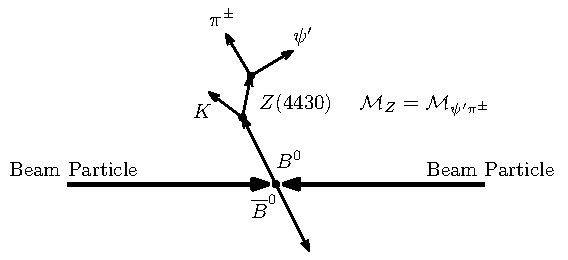
\psfig{file=../figures/Z4430_diagram.pdf, width=0.95\linewidth}}
  \caption{The creation and decay chain of the $Z(4430)$ tetraquark meson.}
  \label{fig:z4430diag}
\end{figure}

Due to the charge of the observed resonance it was impossible for the candidate particle to simply be an exited charmonium state ($c\overline{c}$). Therefore, the observed resonance was a suspected tetraquark state (with quark content $c\overline{c}u\overline{d}$~or $c\overline{c}d\overline{u}$). The $J^P$ of the particle was not measured by Belle, and therefore other hypothesis different from the tetraquark could be made. Another possible state was the $D$ ``molecule.'' A superposition of $D$ meson states forming an isospin multiplet~\cite{z4430_dmolecule}:
\begin{align}
Z^+ &= \frac{1}{\sqrt{2}}\left(D^{*+}\overline{D}^0_1-D^+_1\overline{D}^{*0}\right), \\
Z^0 &= \frac{1}{2}\left(D_1^0\overline{D}^{*0} - D^{*0}\overline{D}_1^0 + D_1^+D^{*-}-D^{*+}D^-_1\right),\\
Z^- &= \frac{1}{\sqrt{2}}\left(D^0_1D^{*-} - D^{*0}D_1^-\right).
\end{align}
Another $B$ factory experiment, BABAR at SLAC, was unable to find the same resonant behavior. Therefore, the official tetraquark discovery was not confirmed by the $B$ factory experiments.

In 2014, the LHCb collaboration at the LHC confirmed the existence of the tetraquark state $Z(4430)^-$ with quark content $c\overline{c}d\overline{u}$~\cite{lhcb}. LHCb confirmed the state at 13.9$\sigma$. The spin-parity of the state was measured to be $J^P = 1^+$, eliminating the possible $D$ molecule and confirming the tetraquark state. The mass and width measured by LHCb are:
\begin{align}
m_{Z^{-}} &= 4475 \pm 7^{+15}_{-25}\text{ MeV},\\
\Gamma_{Z^{-}} &= 172 \pm 13^{+37}_{-34}\text{ MeV}.
\end{align}
Figures~\ref{fig:z4430lhcb1} and ~\ref{fig:z4430lhcb2} show the resonant peak and also the likelihood measurement of for the spin-parity.


\begin{comment}
\begin{figure*}[h!]
  \centerline{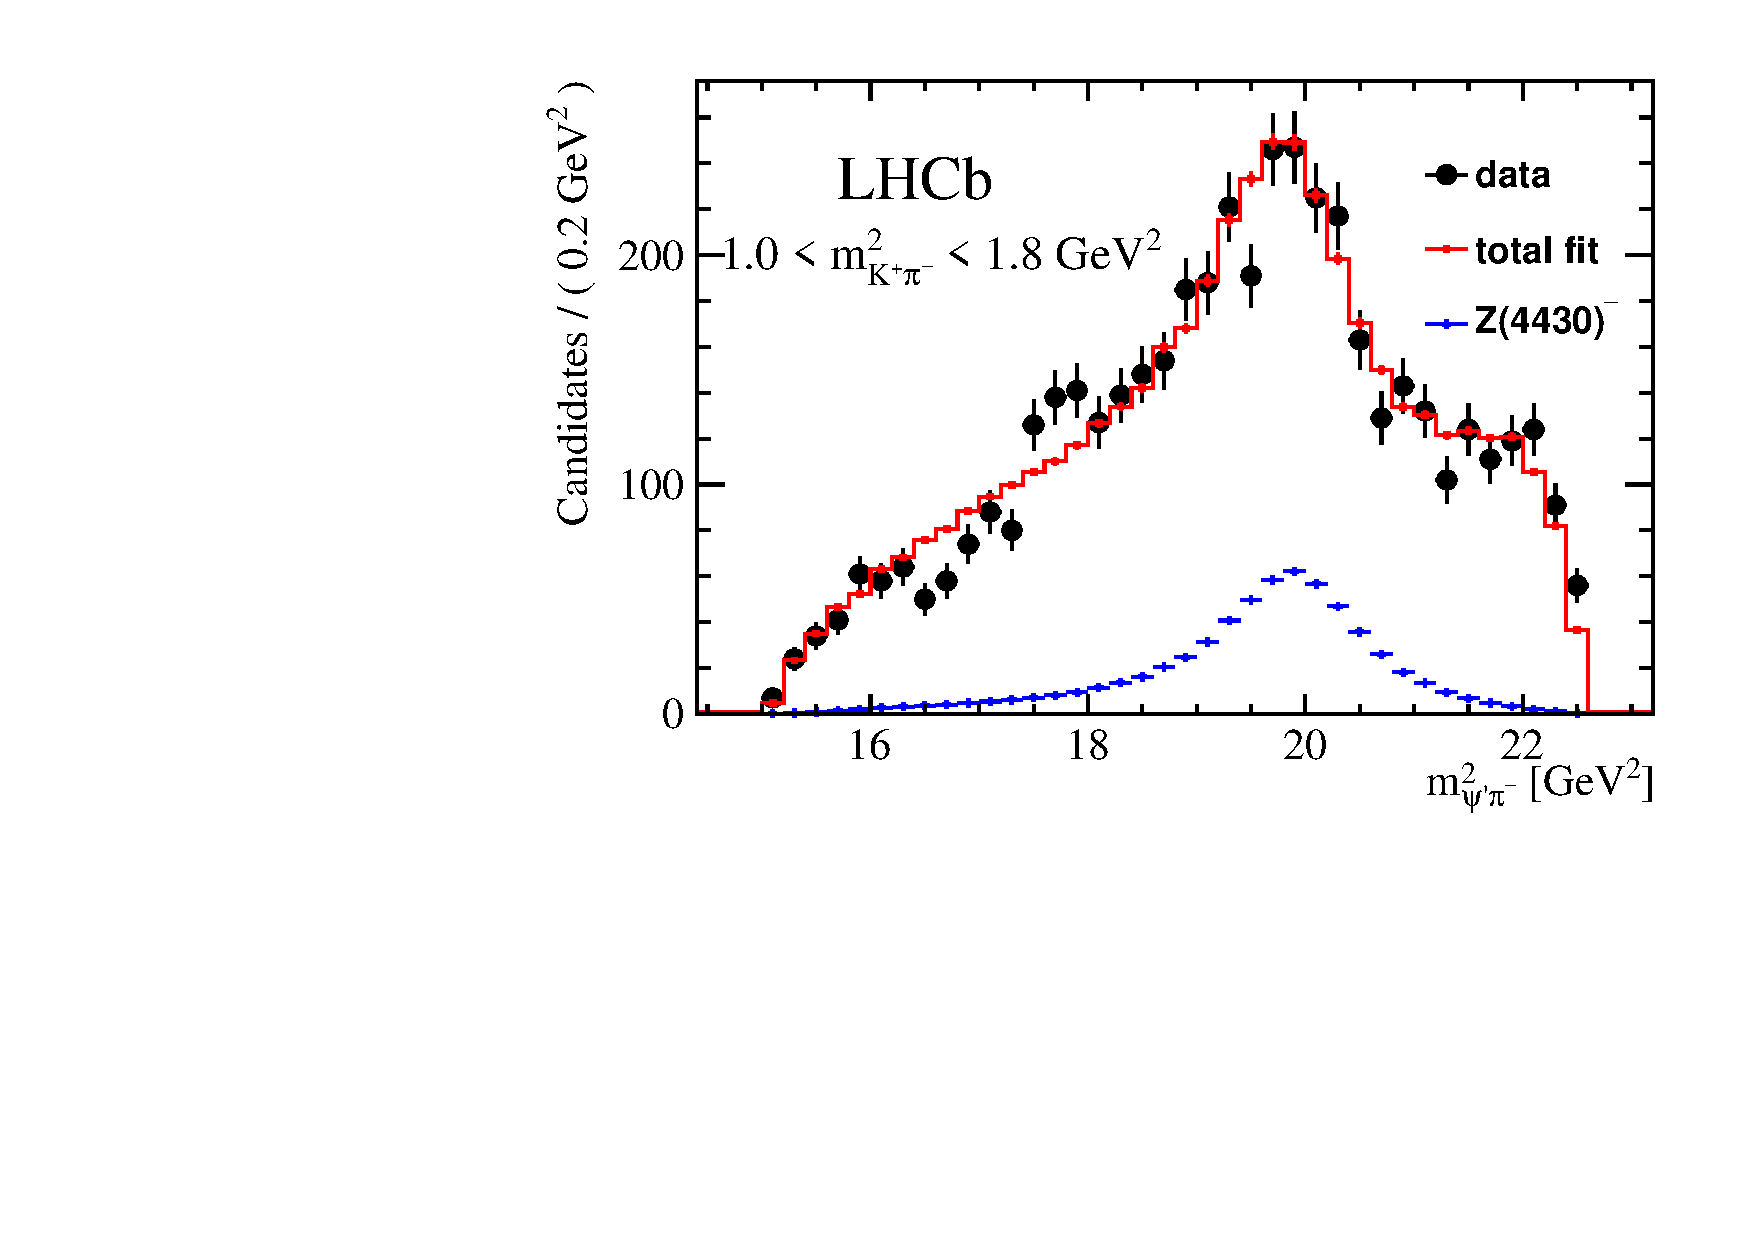
\psfig{file=../figures/Z4430_res.pdf, width=.45\linewidth}
  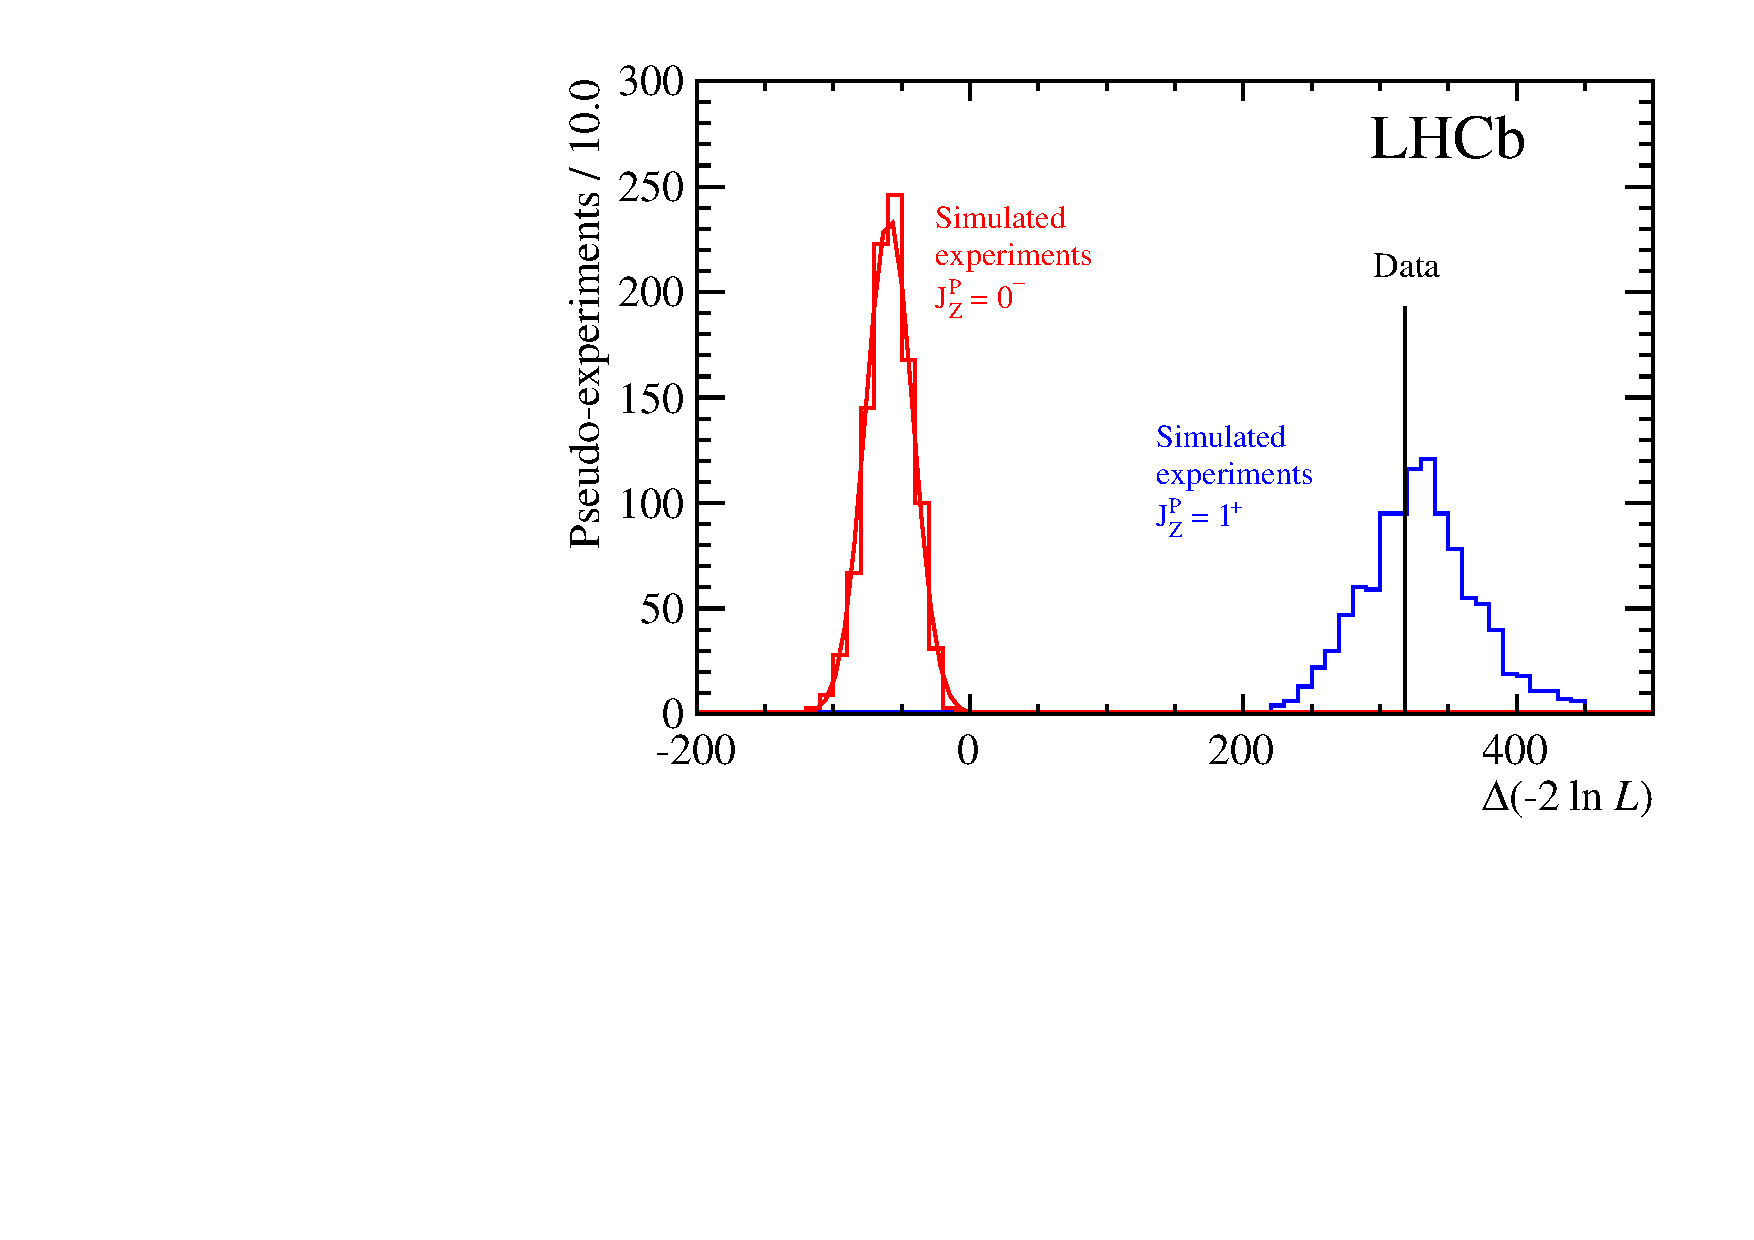
\psfig{file=../figures/Z4430_jp.pdf,width=.45\linewidth}}
  \caption{LHCb plots}
  \label{fig:z4430lhcb}
\end{figure*}
\end{comment}

\begin{figure}[H]
  \centerline{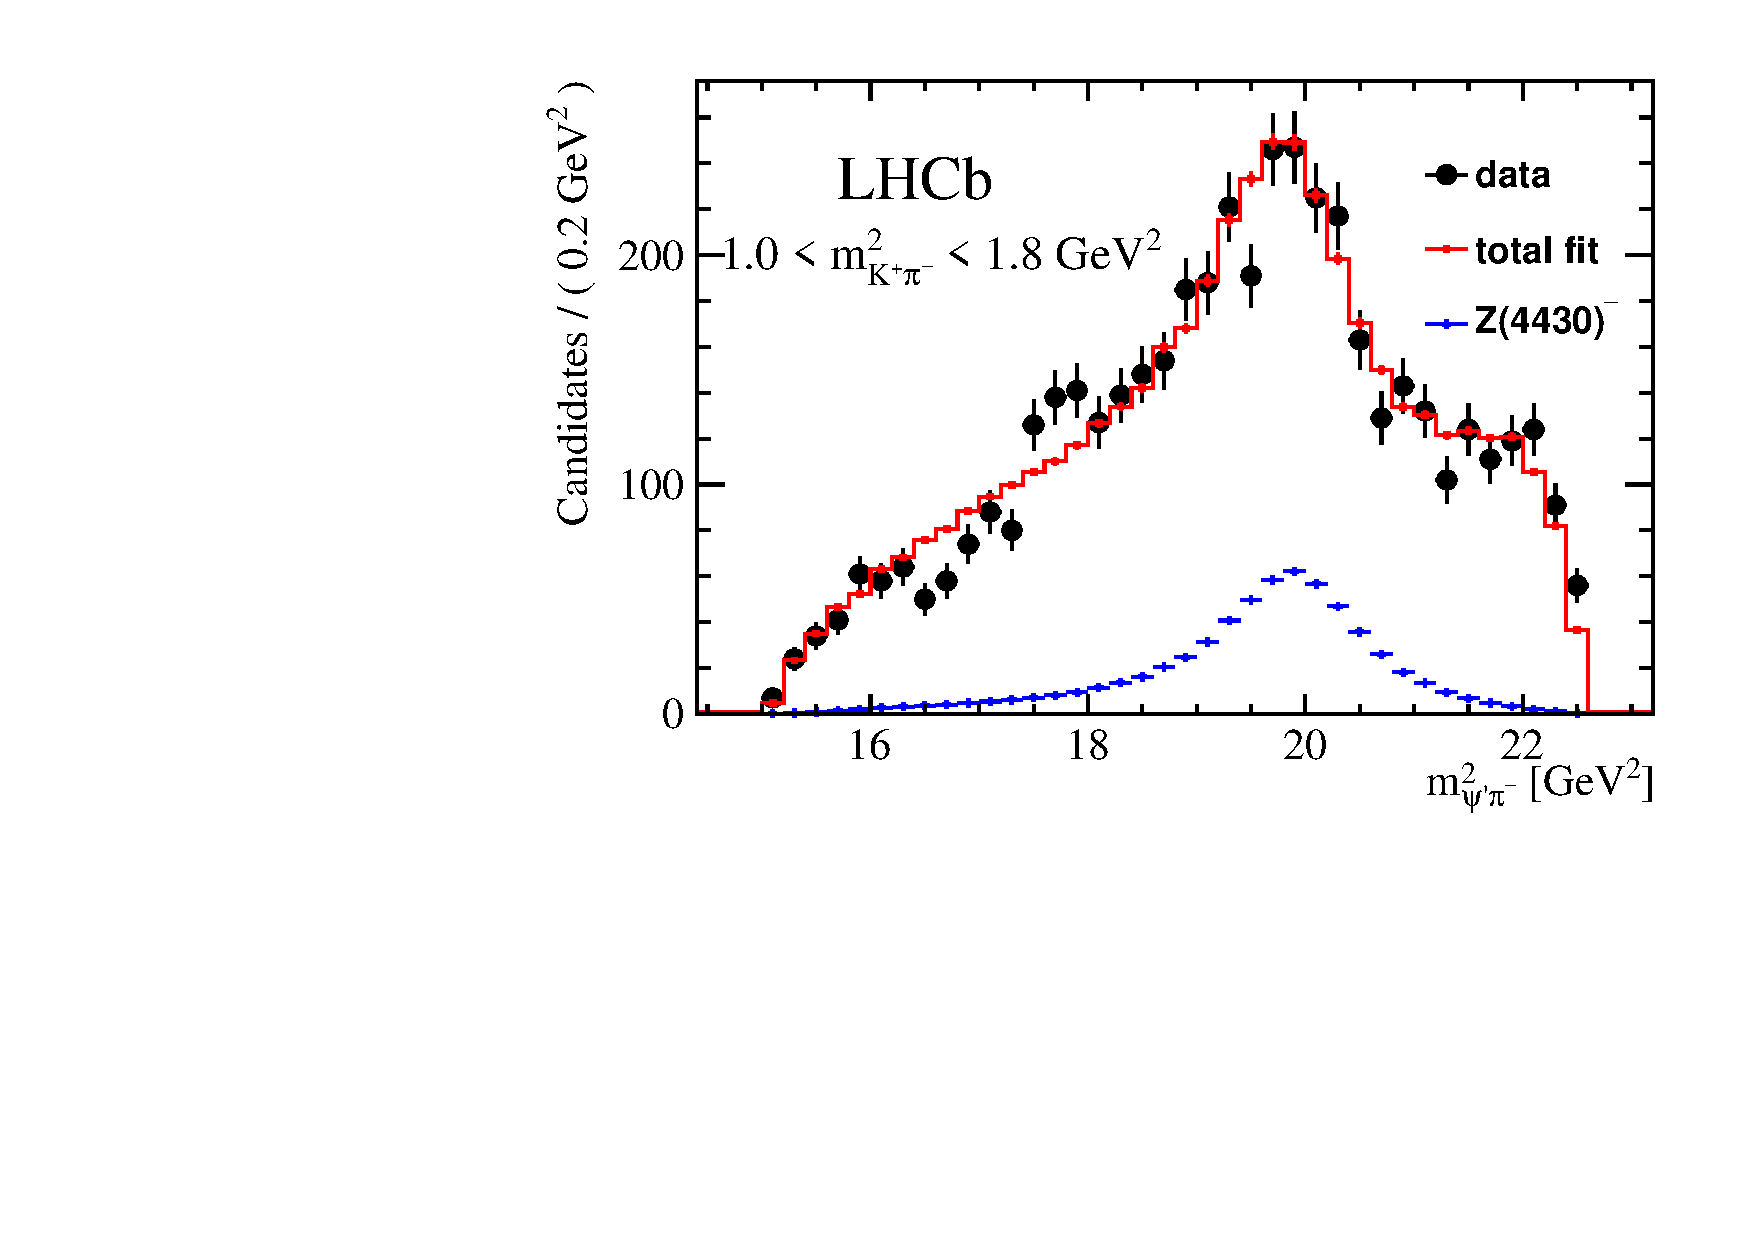
\psfig{file=../figures/Z4430_res.pdf, width=.95\linewidth}}
  \caption{The LHCb measurement of the invariant mass of the $\pi\psi^{\prime}$ system. The peak corresponds to $m=4475$ MeV.}
  \label{fig:z4430lhcb1}
\end{figure}

 \begin{figure}[H]
  \centerline{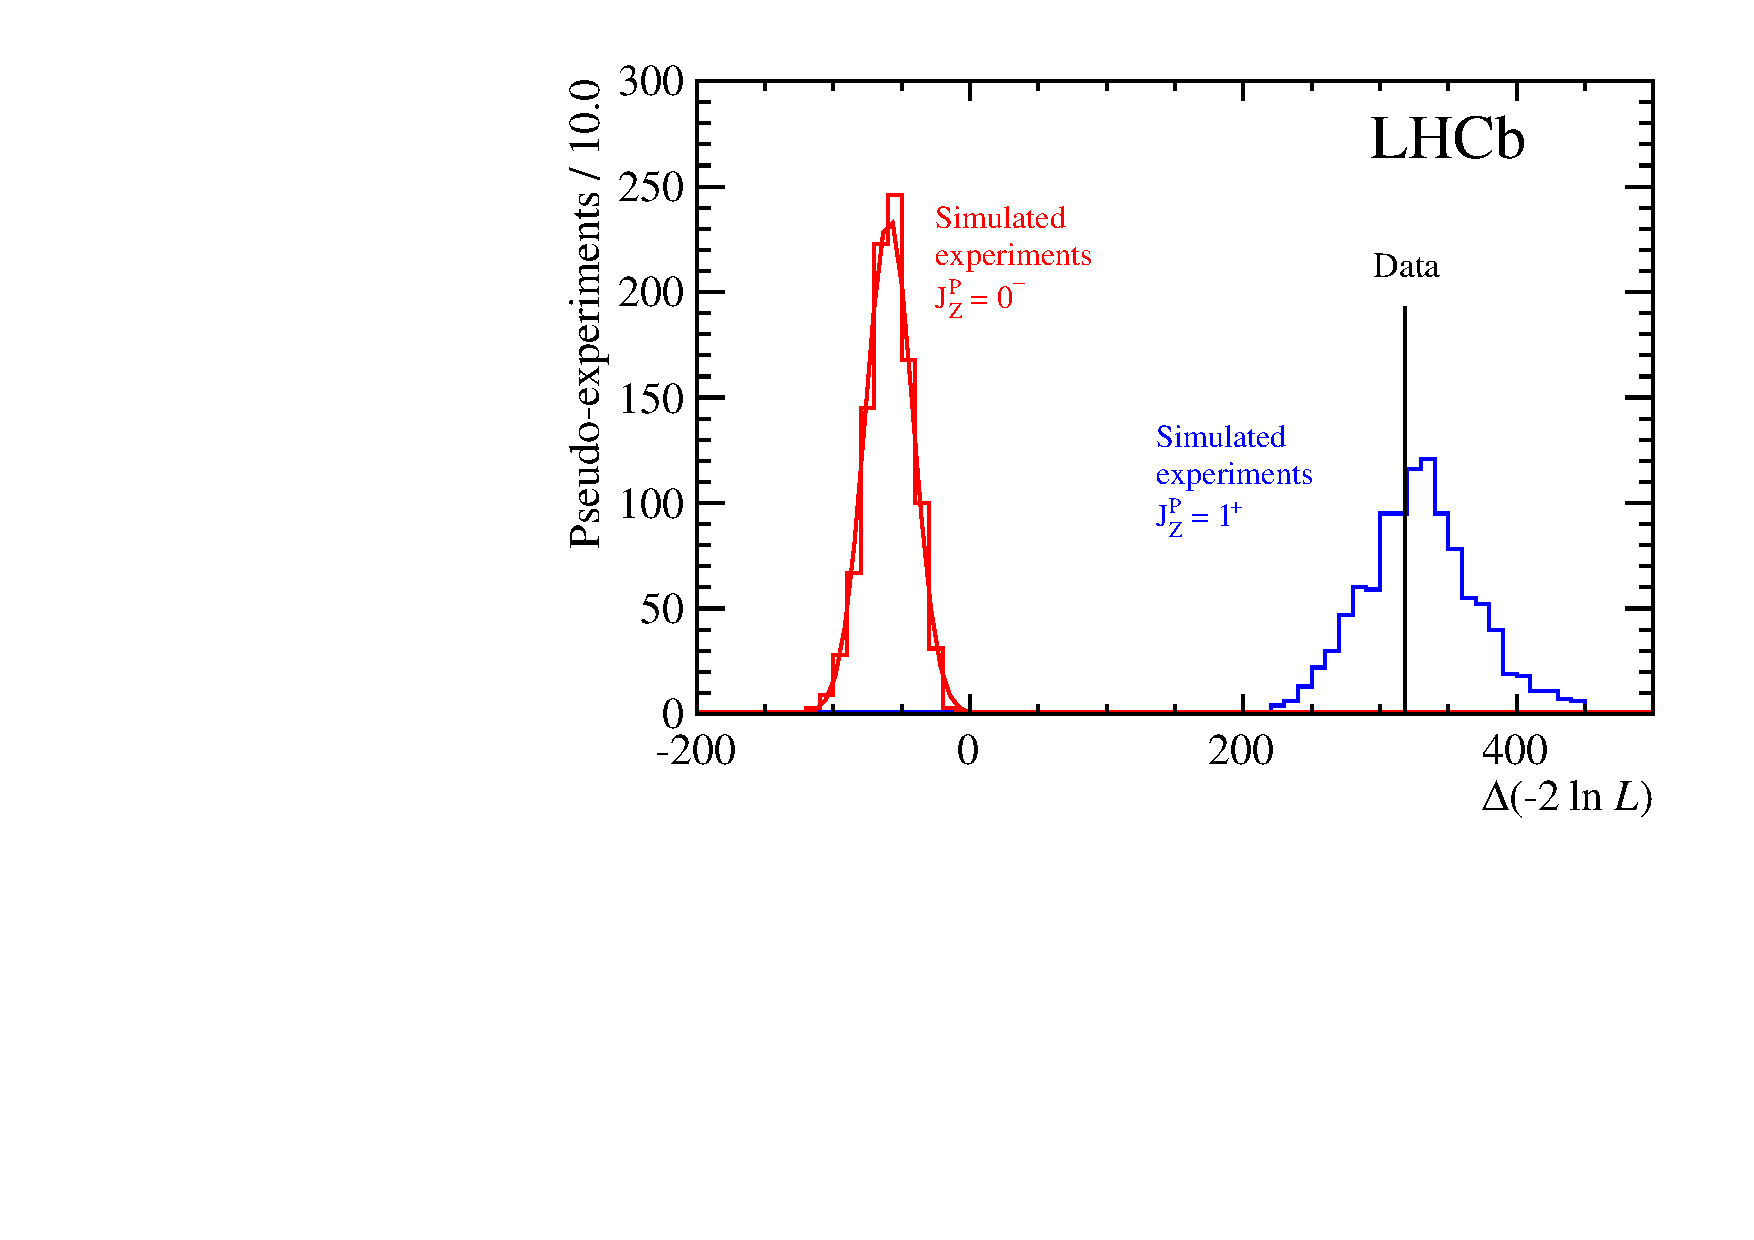
\psfig{file=../figures/Z4430_jp.pdf,width=.95\linewidth}}
  \caption{The LHCb measurement of the spin-parity of the $Z(4430)$.}
  \label{fig:z4430lhcb2}
 \end{figure}


\subsection{$\pi(1400)$ and $\pi(1600)$}
%\todo[inline]{Ping}

Both the Lattice QCD model and the QCD string (QCD flux tube) models predict an exotic hybrid meson with $J^{PC} = 1^{-+}$ with a mass of around 1.9$\pm$0.2 GeV. However, the bag model predicts the exotic $1^{-+}$ at a lower mass of about 1.4 GeV. This exotic $1^{-+}$ meson decaying to $\eta \pi^{-}$, is called $\pi_{1}(1400)$. It is reported in the reaction $\pi^{-}p \rightarrow \eta \pi^{-}p$ at 18.3 GeV by the E852 collaboration using the Multi-Particle Spectrometer (MPS) at the AGS. $\eta$ is detected through $\gamma \gamma$ decay. Evidence of $\pi_{1}(1400)$ is also found in $\pi^{-}p \rightarrow \eta \pi^{0} n$ at 18.3 GeV at E852.

\subsubsection{$p\overline{p}$~Annihilation}

The crystal barrel collaboration at LEAR also searched for a $1^{−+}$ resonance in the $\eta \pi$ P-wave\footnote{Hybrid mesons are expected to predominantly decay into pairs of S and P-wave mesons. The S-wave, angular momentum quantum number $l=0$, corresponds to a classical head on collision. P, $l=1$ and D-waves, $l=2$ have a higher angular momentum between the initial and final states.} in low energy $p\overline{p}$~annihilation into $\pi\pi\eta$. The $\pi_{1}(1400)$ signal is weak in peripheral reactions and contains lots of backgrounds which mimic other 1400 resonances such as the $a_{2}(1320)$ meson; the signal is stronger in $p\overline{p}$~annihilation. Also, a similar $\pi_{1}(1600)$ is also reported both from many peripheral experiments and $p\overline{p}$~annihilation. A confirmation that they are the particle predicted by the flux tube and lattice QCD model requires further theoretical and experimental work.


%\subsection{Implications for Lattice QCD}
%\todo[inline]{??, we need some references on this!!!}

\section{Conclusions}
%\todo[inline]{Justin, Includes short discussion of exotic mesons Implications for Lattice QCD, could just be a rehash of what is said in the hybrids section}
The study of exotic mesons will contribute a great deal to our understanding of QCD. In particular, work on hybrid mesons can eliminate poor lattice QCD models in favor of those that make better experimental predictions. Glueballs and tetraquarks remain elusive, though success in verifying the Z(4430) gives hope that others may soon follow. The field could be a fruitful area of research for some time.


\newpage

\begin{thebibliography}{9}
%\bibitem{Barnes}
%  T. Barnes, \textit{Exotic Mesons, Theory and Experiment}, arXiv:hep-ph/0007296, \url{http://arxiv.org/abs/hep-ph/0007296}
\bibitem{ketzer}
  Bernhard Ketzer, \textit{Hybrid Mesons}, Proceedings of Science, Sixth International Conference on Quarks and Nuclear Physics, PoS(QNP2012)025, \url{http://pos.sissa.it/archive/conferences/157/025/QNP2012_025.pdf} %\url{http://arxiv.org/abs/1208.5125}
%\bibitem{Olsen}
%  Stephen Lars Olsen, \textit{QCD exotics}, Hyperfine Interactions, \textbf{229}, \url{http://dx.doi.org/10.1007/s10751-014-1061-4}
\bibitem{belle}
  S.~K.~Choi~\emph{et. al.}, \emph{Observation of a Resonancelike Structure in the} $\pi^{+-}\psi^{\prime}$ \emph{Mass Distribution in Exclusive} $B\rightarrow K \pi^{+-}\psi^{\prime}$ \emph{Decays}. Phys. Rev. Lett. \textbf{100}, 142001 8 April 2008.
\bibitem{z4430_dmolecule}
  E.~Braaten~and~M.~Lu, \emph{Line shapes of the Z(4430)} Phys. Rev. D \textbf{79} 051503(R) 11 March 2009
\bibitem{lhcb} % {j4}
  LHCb Collaboration, R. Aaij \textit{et al.}, \textit{Observation of the Resonant Character of the }$Z(4430{)}^{-}$\textit{ State}, Phys. Rev. Lett., \textbf{112}, 22 (2014). \url{http://dx.doi.org/10.1103/PhysRevLett.112.222002}%\url{http://link.aps.org/doi/10.1103/PhysRevLett.112.222002}


\bibitem{j1}
 K.A. Olive \textit{et al.} (Particle Data Group), \textit{Non--\qqbar~Mesons} (Revised March 2006 by C. Amsler), Chin. Phys. C, 38, 090001 (2014), \url{http://pdg.lbl.gov/2006/reviews/nonqqbar_mxxx050.pdf}
\bibitem{j2}
 Vincent Mathieu, Nikolai Kochelev, and Vicente Vento, \emph{The Physics of Glueballs}, Int. J. Mod. Phys. E \textbf{18}, 1 (2009), \url{http://www.worldscientific.com/doi/abs/10.1142/S0218301309012124}
\bibitem{j3}
 Wolfgang Ochs, \emph{The status of glueballs}, J. Phys. G: Nucl. Part. Phys. \textbf{40}, 043001 (2013), \url{http://dx.doi.org/10.1088/0954-3899/40/4/043001}


\end{thebibliography}

\end{document} %%% end of doc %%%

%%%%%%%%%%%%%%%%%%%%%%%%%%%%%%%%%
%%%%%%%%%%%%%%%%%%%%%%%%%%%%%%%%%
%%%%%%%%%%%%%%%%%%%%%%%%%%%%%%%%%
%%%%%%%%%%%%%%%%%%%%%%%%%%%%%%%%%

\section{Simulation and Results}
\subsection{Simulation Setup}

Modifications to the example for our project include changes to the \texttt{PrimaryGeneratorAction}, \texttt{PhysicsList} \texttt{DetectorConstruction}, \texttt{RunAction}, and \texttt{EventAction}. For the generation of particles, we change the energy of the incoming particle, and also vary the particle type. We use electrons, muons, protons, and neutrons. For the detector construction, we create what is essentially a single block of material, with eight independent ``channels.'' When the particle propagates through the detector, it is always going through the same material, but independent layer by layer hit information is created by declaring eight different \texttt{LogicalVolume} objects.\footnote{For further discussion of volumes in Geant4 see Appendix~\ref{sec:AppendixA}} At the beginning of the \texttt{RunAction}\footnote{For further discussion of run and event actions, see Appendix~\ref{sec:AppendixB}} a ROOT~\cite{ROOT} \texttt{TFile} is initialized along with a \texttt{TTree} for data output. Sixteen branches are created for storing the energy deposited and track length for each layer. In the \texttt{EventAction}, \texttt{G4HitsCollection} pointers are declared to retrieve the total energy deposited and track length in each layer. These objects are pulled from the \texttt{G4SensitiveDetector} Manager. A pointer to the \texttt{RunAction} is declared in the \texttt{EventAction} where the function \texttt{RunAction::UpdateTree} has the current event's energy deposition and track length values updated in the \texttt{RunAction}, filling the whole run's \texttt{TTree}. At the end of the number of requested events, the \texttt{RunAction::EndOfRunAction} function writes the ROOT \texttt{TTree} to the \texttt{TFile} and closes the \texttt{TFile}.

\subsection{Event Visualizations and Qualitative Event Analysis}


\begin{figure*}
  \centering
  \subfloat[Electron events \label{fig:e-geo}]
  {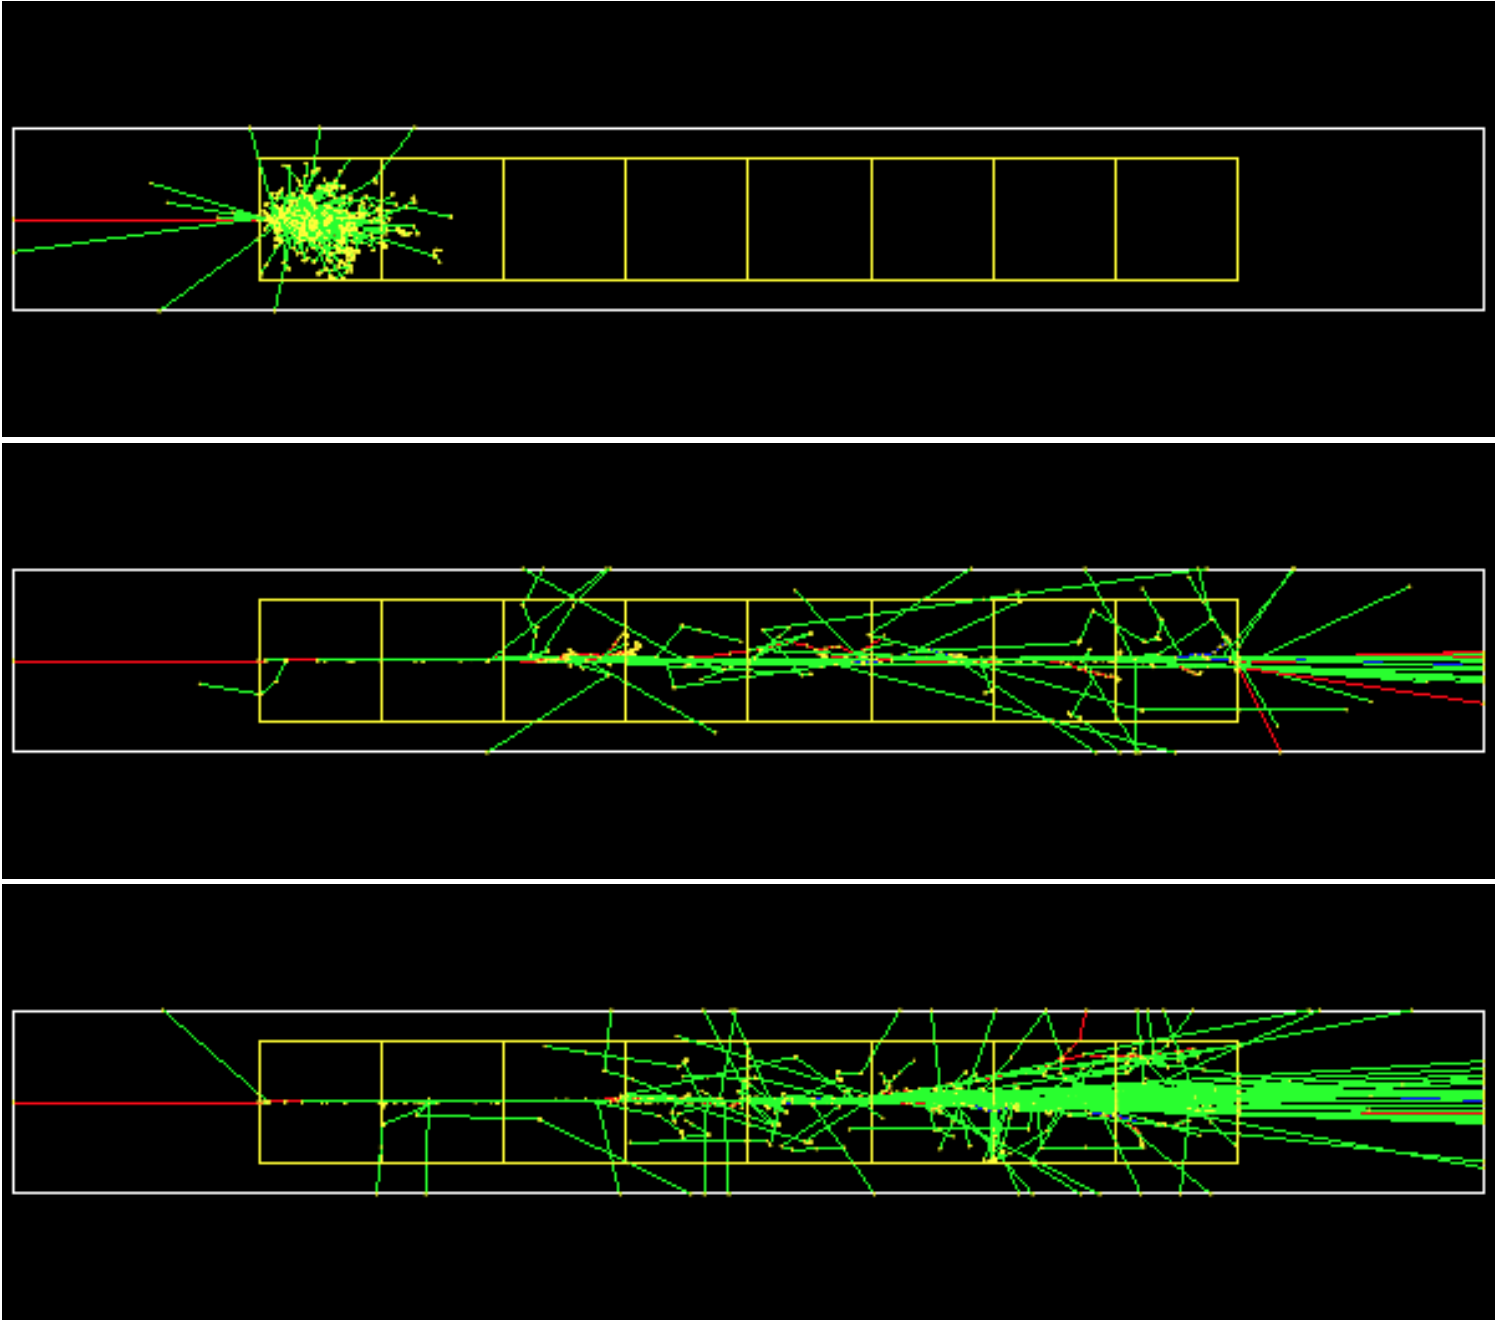
\includegraphics[width=0.44\textwidth]{pics/electron_ed.png}}
  \hfill
  \subfloat[Muon events \label{fig:mu-geo}]
  {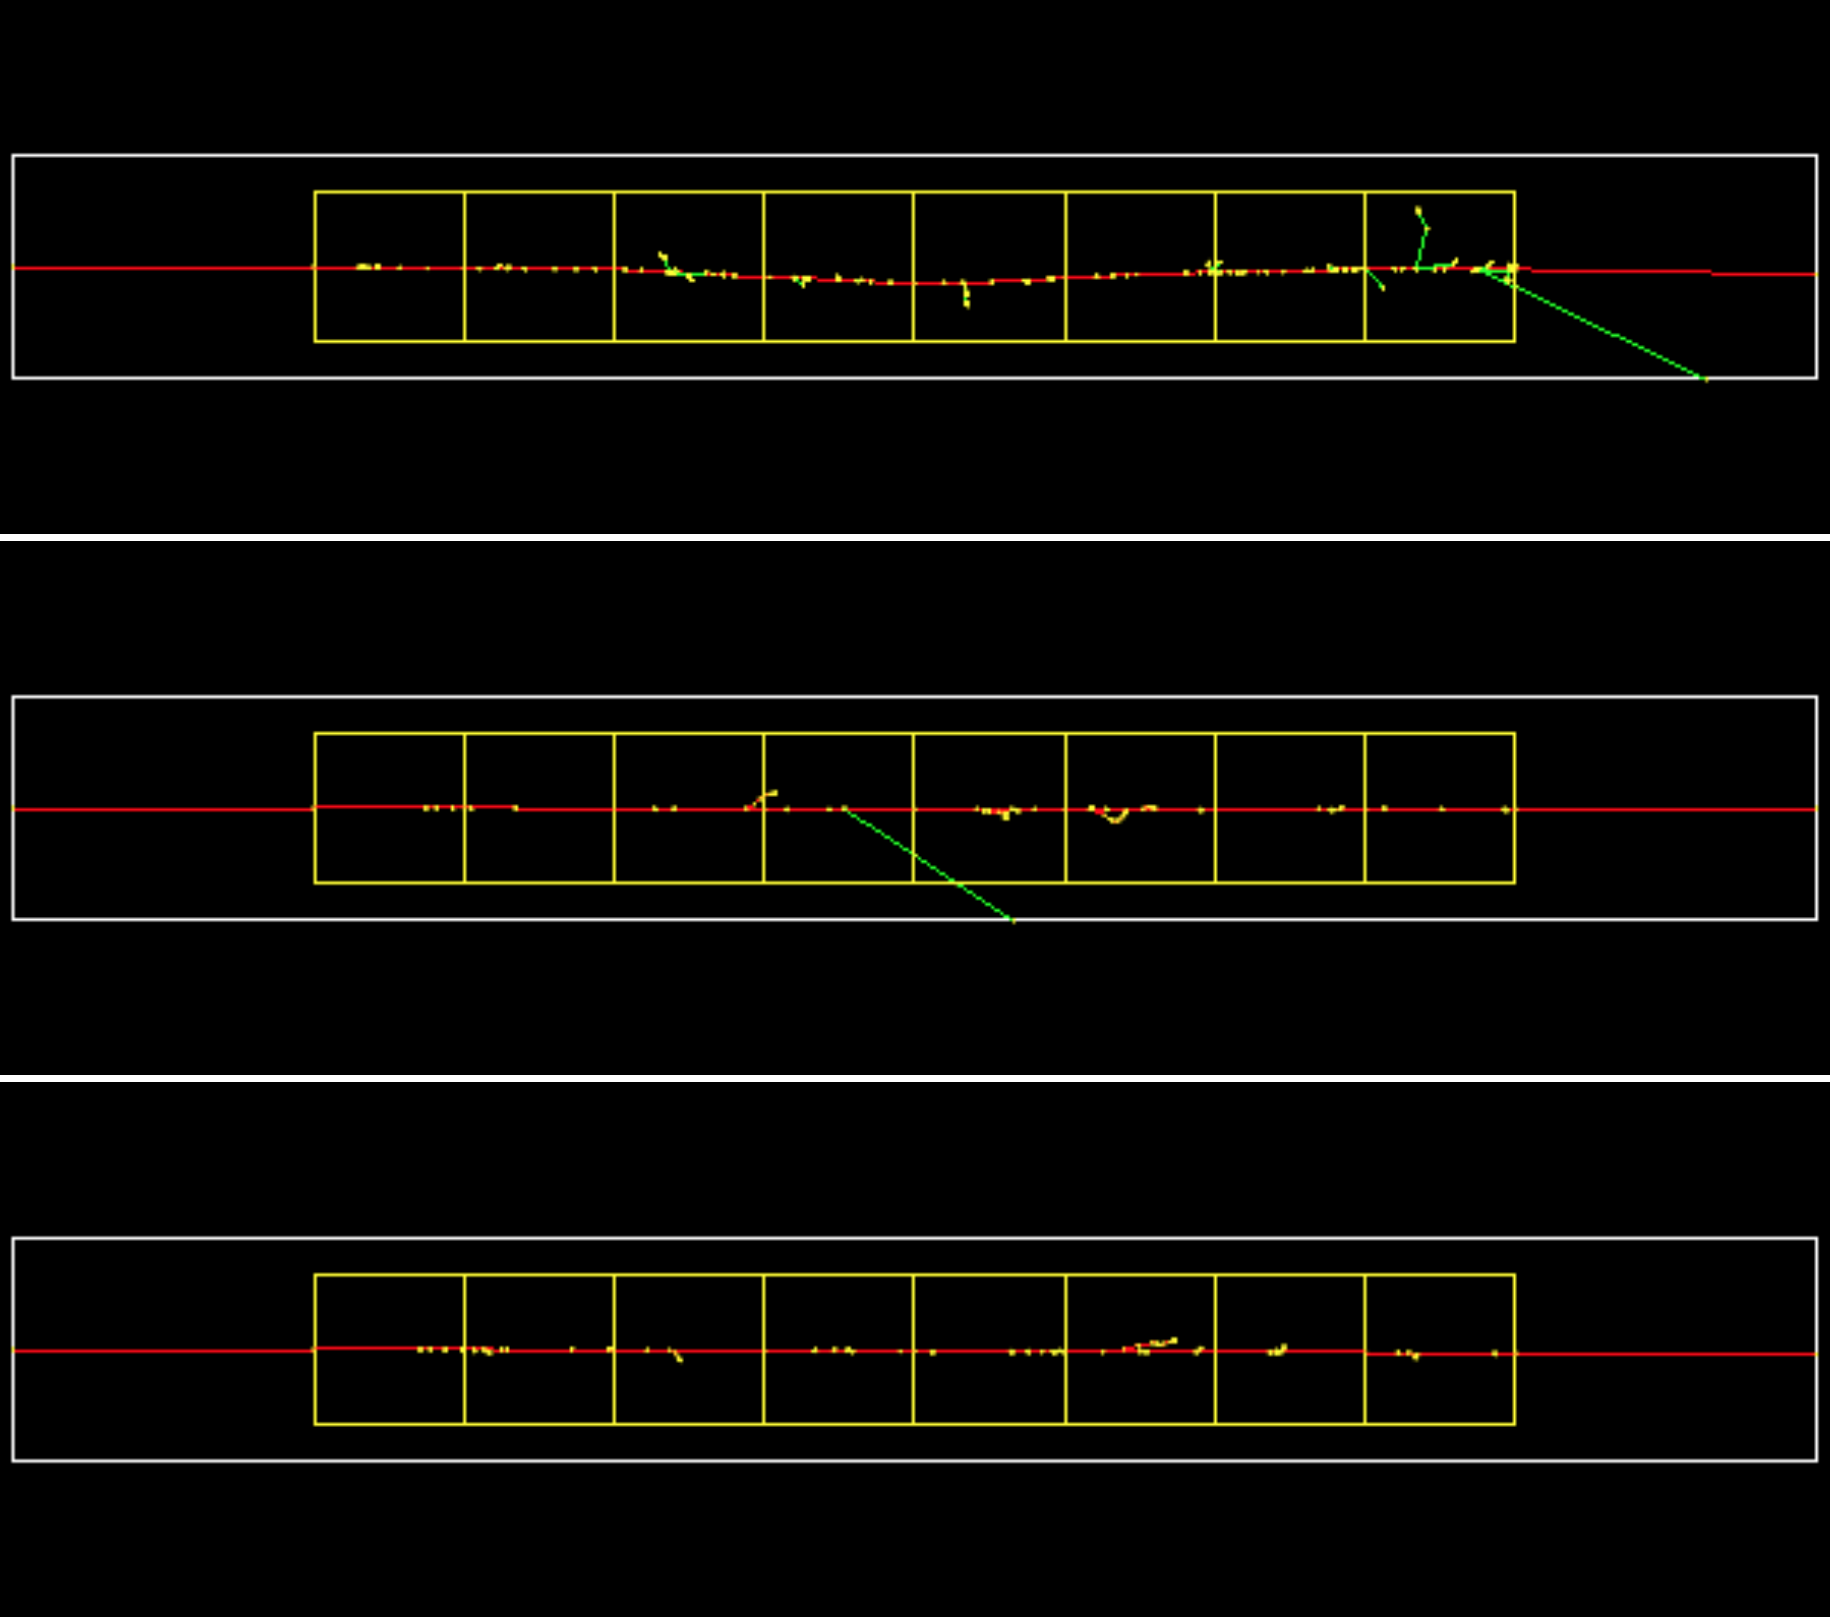
\includegraphics[width=0.44\textwidth]{pics/muon_ed.png}}
  \hfill
  \subfloat[Proton events \label{fig:P-geo}]
  {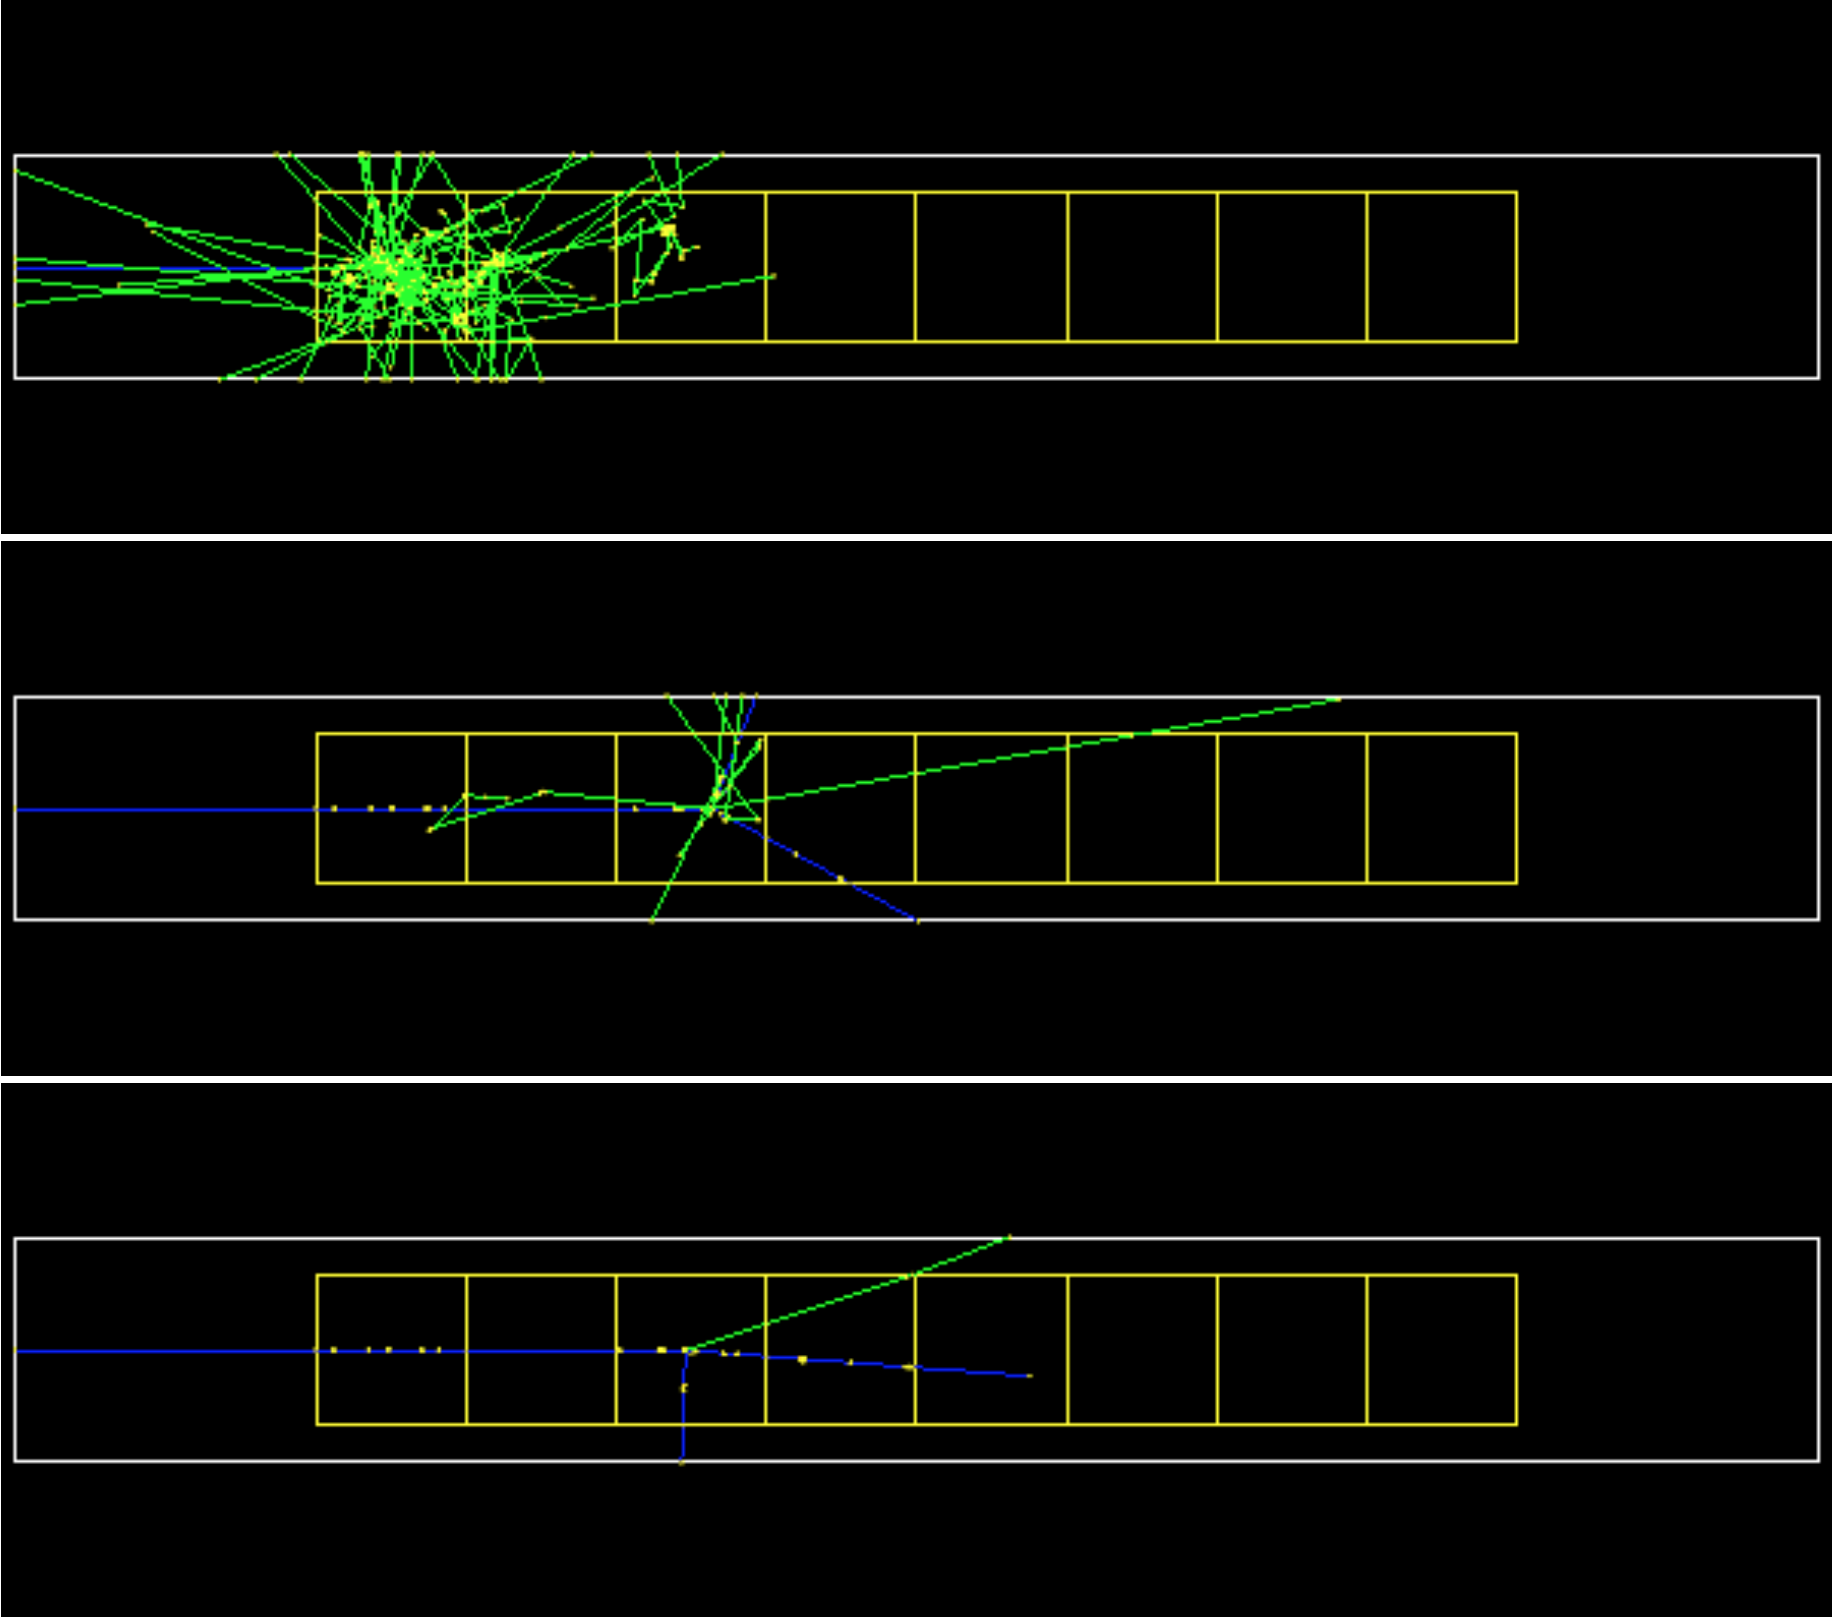
\includegraphics[width=0.44\textwidth]{pics/proton_ed.png}}
  \hfill
  \subfloat[Neutron events \label{fig:N-geo}]
  {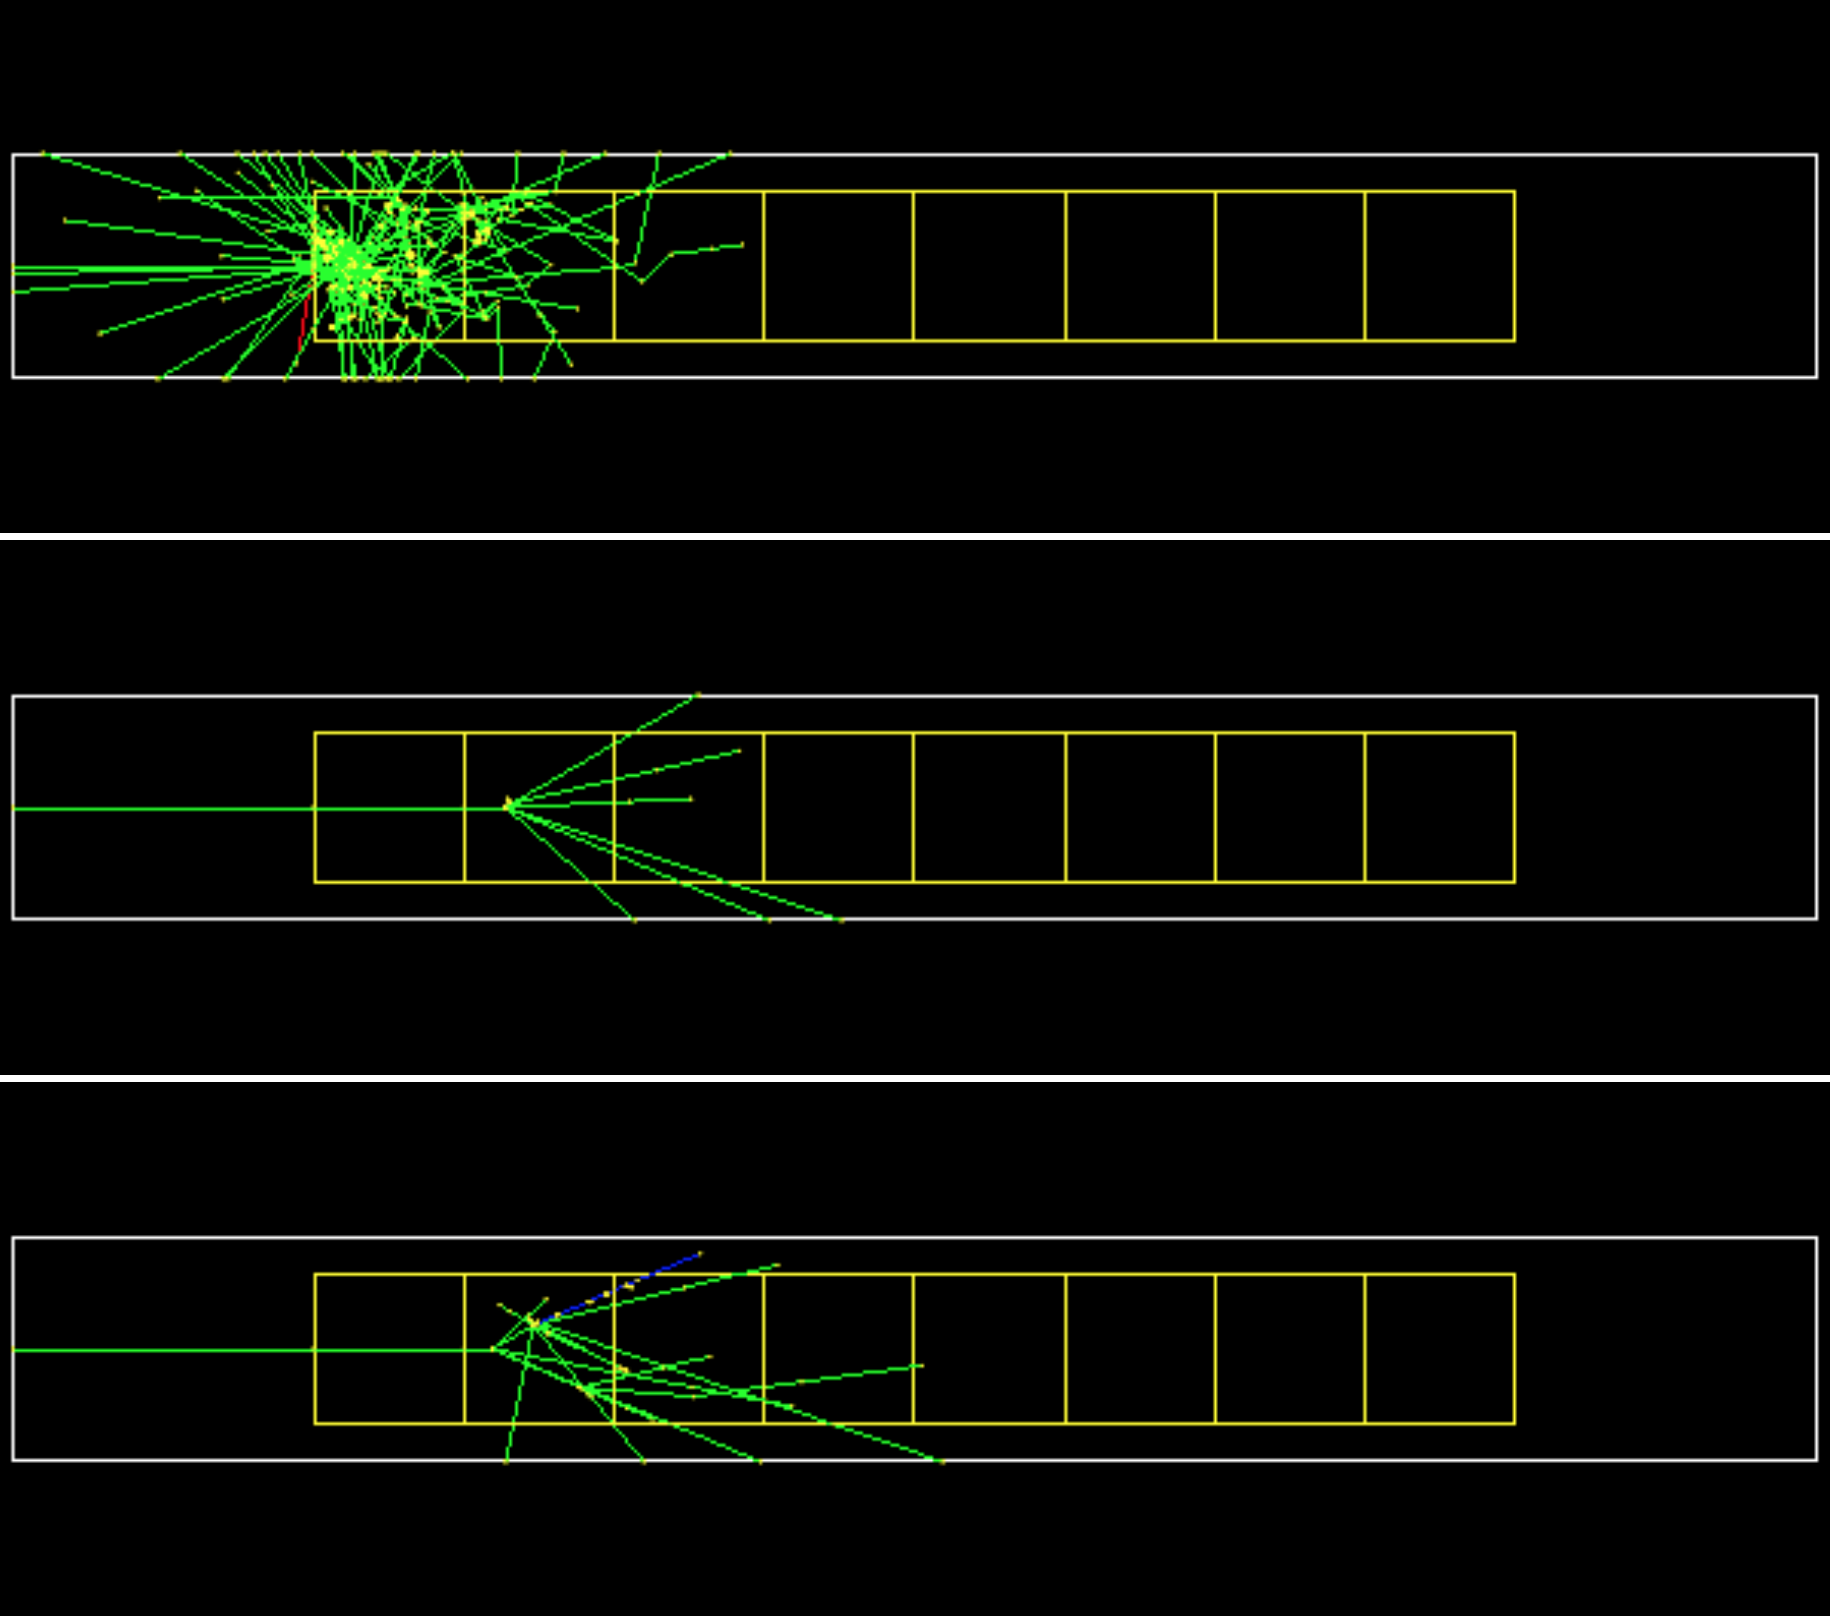
\includegraphics[width=0.44\textwidth]{pics/neutron_ed.png}}
  \caption{The detector geometry with a 2 GeV particle events in three different materials. The top displays corresponds to lead, the middle displays to polypropylene, and the bottom displays to water. Red trajectories indicate negatively charged tracks, green neutral tracks, and blue positively charged tracks.}
  \label{fig:mean and std of nets}
\end{figure*}

\begin{appendix}

\section{Volumes in Detector Construction}\label{sec:AppendixA}

\end{appendix}


